\subsection{Durchführung des Großtests 1}

Der Test wurde 31.08.2015 durchgeführt. Eine Durchführung zu einem früheren Zeitpunkt war nicht möglich, da erst in Sprint 8 das Routing implementiert wurde.
Die Handys wurden mit Buchstaben benannt und in Raum C205 verteilt.


\subsubsection{Ergebnisse Test 1}

Wir haben auf 117 Nachrichten 11 erfolgreiche Fälle und 106 Errors.

\paragraph{Folgende Beispiele veranschaulichen Nachrichten, die beim Empfänger angekommen sind:}

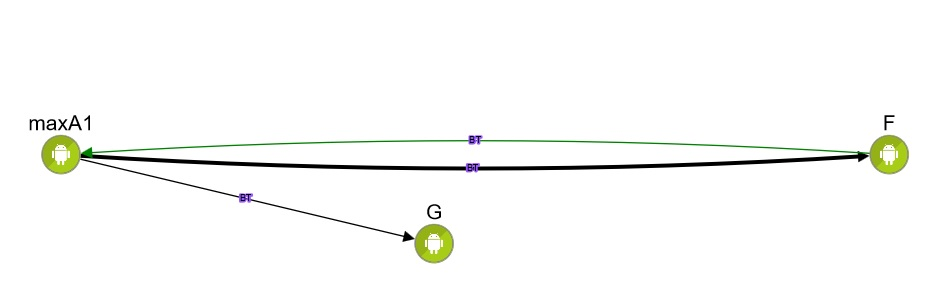
\includegraphics[width=1.0\textwidth]{belege/grosstests/Bilder/Erfolg4.jpg}\\
1. A sendet eine Nachricht an F. A sendet die Nachricht an G und F los, da A nur den
Bluetooth Namen der Handys kennt, und so nicht weiß, dass F sich in
Reichweite befindet. F sendet ein Acknowledgement zurück, während G die
Nachricht nicht weiterleiten kann.\\
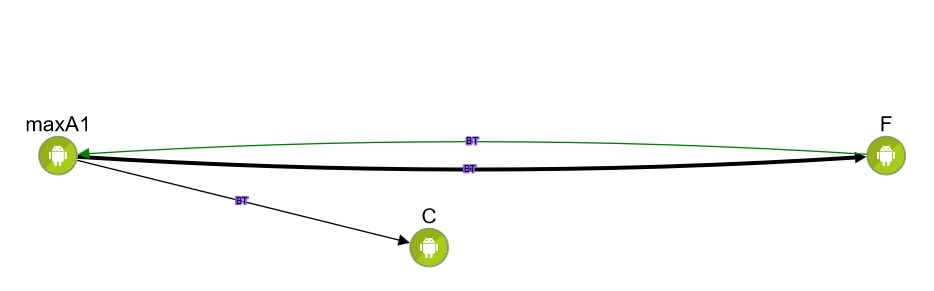
\includegraphics[width=1.0\textwidth]{belege/grosstests/Bilder/Erfolg3.jpg}\\
2. Gleiches Szenario wie in 1, nur diesmal mit C statt G.\\
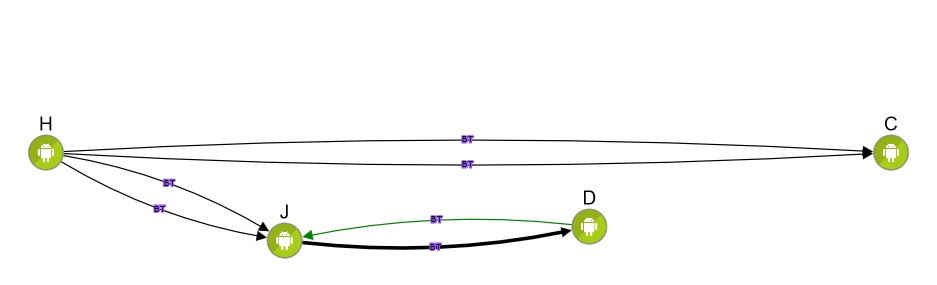
\includegraphics[width=1.0\textwidth]{belege/grosstests/Bilder/Erfolg2.jpg}\\ 3. H sendet eine
Nachricht an D. Es befinden sich J und C in Reichweite. C leitet die
Nachricht nicht weiter. J hat jedoch eine Verbindung zu D. D sendet ein
Acknowledgement über den Pfad, über den er die Nachricht empfangen hat,
zurück.\\ 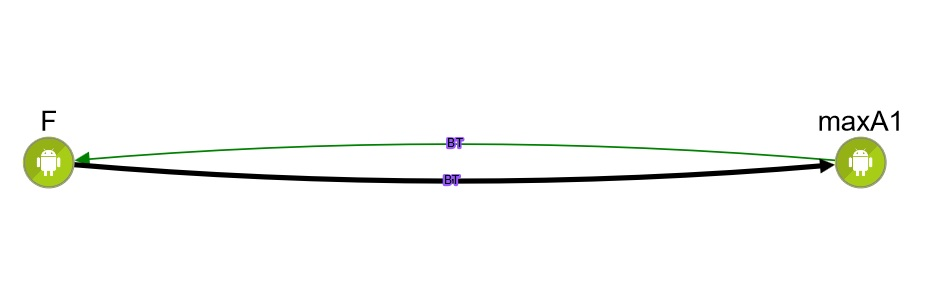
\includegraphics[width=1.0\textwidth]{belege/grosstests/Bilder/Erfolg1.jpg} \\4. Eine
erfolgreich übertragene Nachricht zwischen 2 benachbarten Handys mit
Acknowledgement.

\paragraph{Folgende Beispiele veranschaulichen Nachrichten, die nicht beim Empfänger angekommen sind:}
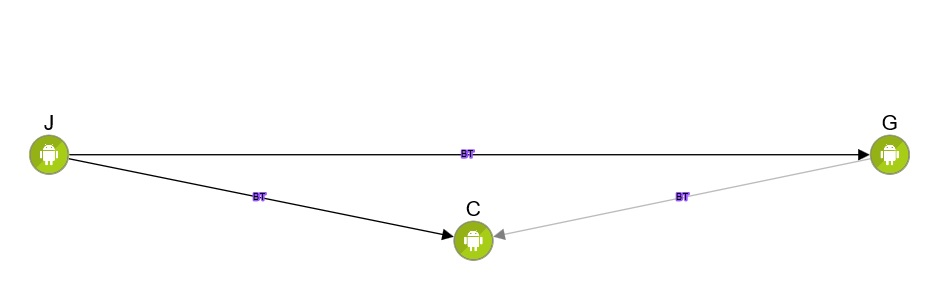
\includegraphics[width=1.0\textwidth]{belege/grosstests/Bilder/Miserfolg6.jpg}\\ 1. J versucht
eine Nachricht zu schicken. Es befinden sich jedoch nur die Handys G und
C in Reichweite, die jedoch nicht der Empfänger sind. G kann daraufhin nur Verbindung mit C herstellen, das
jedoch die Nachricht bereits kennt.\\
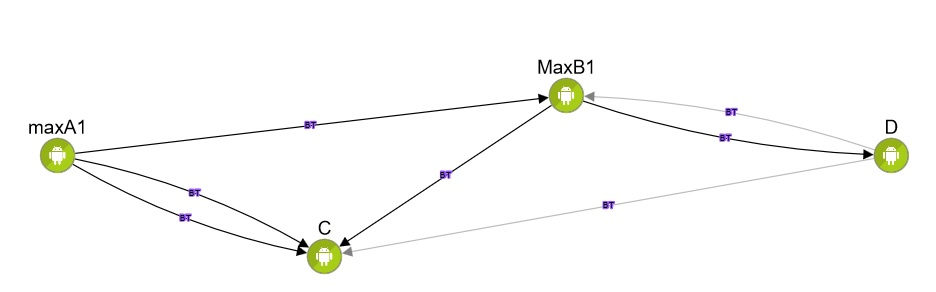
\includegraphics[width=1.0\textwidth]{belege/grosstests/Bilder/Miserfolg5.jpg}\\ 2. A versucht
eine Nachricht zu schicken. Es befinden sich jedoch nur die Handys B und
C in Reichweite. B kann die Nachricht nun noch an D weiterleiten. Dort
bleibt sie jedoch hängen, da D nur noch eine Verbindung zu C findet, das
die Nachricht bereits kennt. A versucht daraufhin in einem Retry die
Nachricht erneut zu schicken, findet aber nun nur noch C.\\
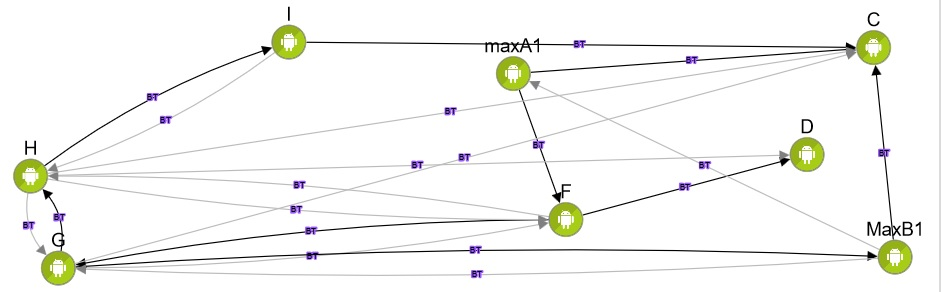
\includegraphics[width=1.0\textwidth]{belege/grosstests/Bilder/Miserfolg4.jpg}\\ 3. An diesem
Beispiel erkennt man, dass alle Handys nah zueinander lagen. Die
Nachricht wird von A verschickt. Sie durchläuft sieben der neun anderen Handys.\\
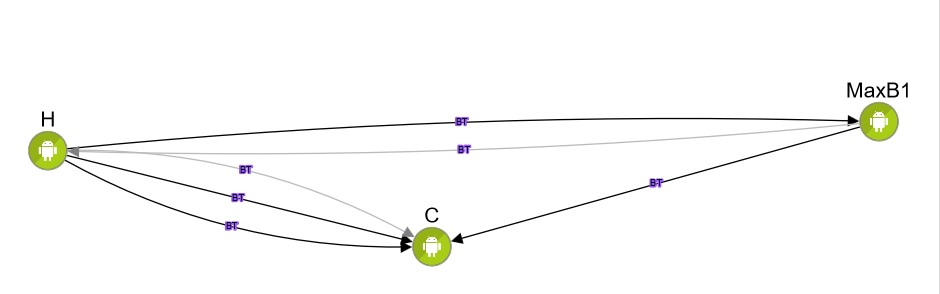
\includegraphics[width=1.0\textwidth]{belege/grosstests/Bilder/Miserfolg3.jpg}\\ 4. H versendet
diese Nachricht. Handy C blockiert jedoch die erfolgreiche Übermittlung
der Nachricht. \\
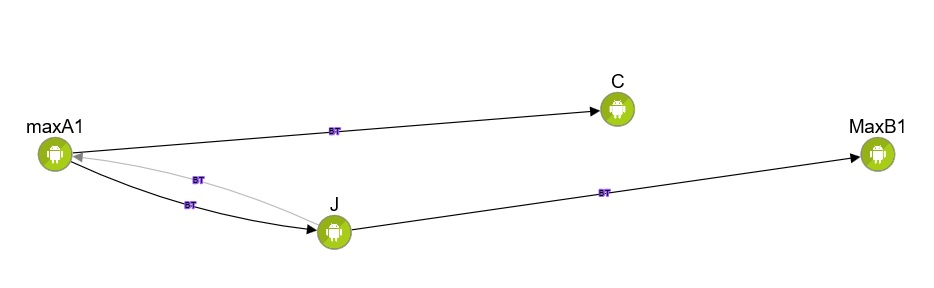
\includegraphics[width=1.0\textwidth]{belege/grosstests/Bilder/Miserfolg2.jpg}\\
5. Auch hier kommt die Nachricht nicht an Handy C vorbei. Auf einem
anderem Pfad schafft sie zwei Hops.\\
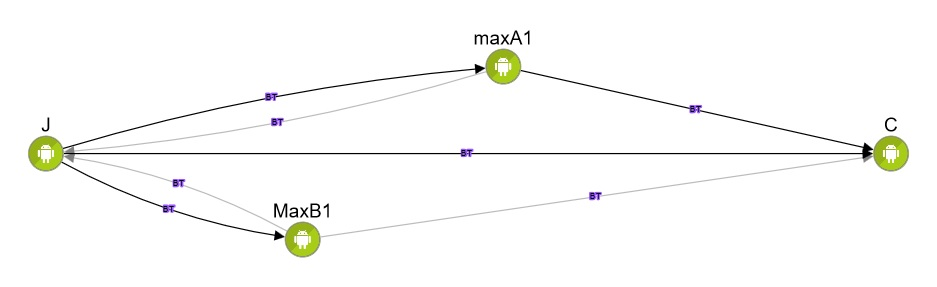
\includegraphics[width=1.0\textwidth]{belege/grosstests/Bilder/Miserfolg1.jpg}\\ 6. J versendet
hier die Nachricht an seine drei Nachbarn. Da jedoch J, A und B (nur) C als
Nachbarn finden, kommt die Nachricht nicht an.\\

\paragraph{Schlussfolgerung aus dem Test:}

Es kamen extrem wenige Nachrichten an. Dies lag daran, dass die Handys
Probleme hatten, sich zu verbinden. Es liegt nahe, dass der
Bluetoothadapter nicht genügend Ports hat um sich mit allen in der Nähe
befindlichen Geräten zu verbinden. Eine Möglichkeit dies zu lösen, wäre
es, sich nicht dauerhaft mit allen Geräten in der Umgebung zu verbinden,
sondern eine Verbindung nach einer Übertragung wieder zu schließen.

Weiterhin gab es Handys, die Nachrichten überhaupt nicht
weitergeleitet haben. Vermutlich war an diesen der Stromsparmodus von
Android aktiv. Ein Beispiel hierfür wäre C.

\paragraph{Verbesserungen bis zum nächsten Test:}

\begin{itemize}
  \tightlist
  \item Die Anzahl der aufzubauenden Verbindungen heruntersetzen.
  \item Ein Test mit mehr anwesenden Personen durchführen um Android daran zu hindern in den Stromsparmodus zu gehen, da dieser nicht ohne Root-Rechte abschaltbar ist.
\end{itemize}


\subsubsection{Ergebnisse Test 2}

Bevor wir Test 2 gestartet haben, haben wir auf allen Handys den
Bluetooth Adapter deaktiviert und erneut aktiviert. Das sollte
eingefrorene Bluetooth Adapter wieder aktivieren. Dieses Vorgehen
basierte auf Erfahrungen von früheren kleinen Tests beim Programmieren.

Im Test 2 haben wir auf 166 Nachrichten 2 erfolgreiche Fälle und 164
Errors.

\paragraph{Folgende Beispiele veranschaulichen die Nachrichten, die beim
Empfänger angekommen sind:}

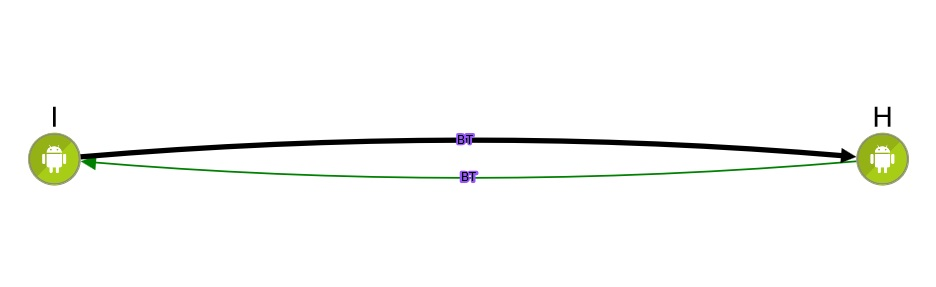
\includegraphics[width=1.0\textwidth]{belege/grosstests/Bilder/Test2Erfolg1.jpg}\\
 1. Nachricht
zwischen zwei benachbarten Handys.\\
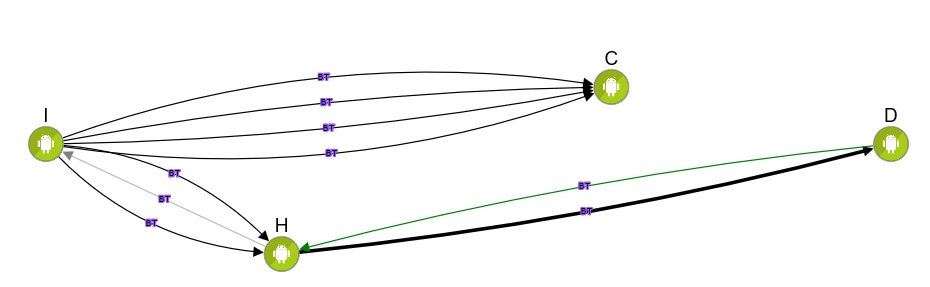
\includegraphics[width=1.0\textwidth]{belege/grosstests/Bilder/Test2Erfolg2.jpg}\\ 2. Nachricht
über einen Hop, die bei einem Retry erfolgreich wurde.\\

\paragraph*{Folgende Beispiele veranschaulichen Nachrichten, die nicht beim
Empfänger angekommen sind:}

\includegraphics[width=1.0\textwidth]{belege/grosstests/Bilder/Test2Misserfolg1.jpg}\\ 1. Das
Handy J hatte während des kompletten Tests keine Verbindung zu einem
Handy aufbauen können.\\
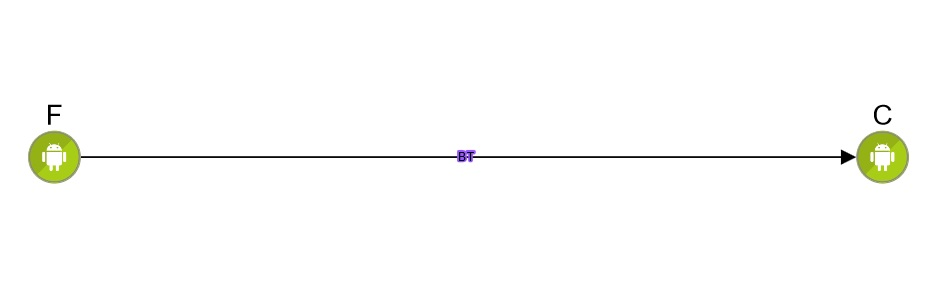
\includegraphics[width=1.0\textwidth]{belege/grosstests/Bilder/Test2Misserfolg3.jpg}\\ 2.
Generell hatten die Handys mehr Probleme Verbindungen aufzubauen.
Dadurch gab es viele Nachrichten, die gar nicht, oder nur bis zum
Nachbarn weitergeleitet wurden.\\
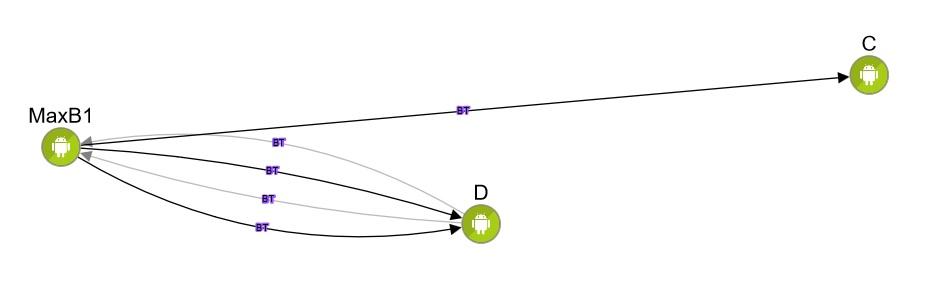
\includegraphics[width=1.0\textwidth]{belege/grosstests/Bilder/Test2Misserfolg4.jpg} \\3. Das
Handy B versucht eine Nachricht zu verschicken, schafft es jedoch nur
bis zu seinen unmittelbaren Nachbarn.\\
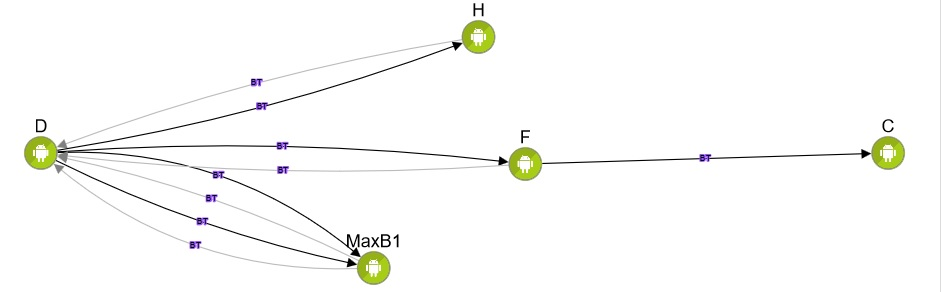
\includegraphics[width=1.0\textwidth]{belege/grosstests/Bilder/Test2Misserfolg5.jpg}\\
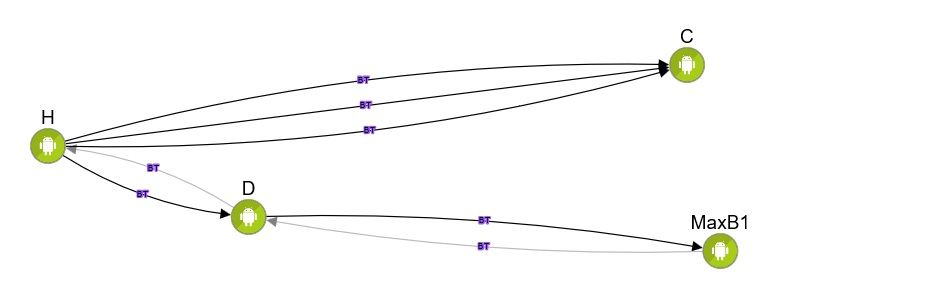
\includegraphics[width=1.0\textwidth]{belege/grosstests/Bilder/Test2Misserfolg6.jpg}\\ 4. und
5. Nachrichten wurden von einem Handy verschickt und schafften es eine
Nachricht mehr als einen Hop zu übertragen. Dies passierte bei diesem
Test bereits sehr selten.\\

\paragraph{Schlussfolgerung aus dem Test:}

Dieser Test zeigte, dass bereits Abstände von circa 5 Metern einen stark
beeinflussenden Faktor haben und extrem viel weniger Verbindungen
aufgebaut wurden als in Test 1.\\

Auch hier gab es wieder Handys, die vermutlich von Android in den
Energiesparmodus versetzt wurden, da diese von niemandem bedient wurden
und nur als Relaisstation gedient haben.

\paragraph{Verbesserungen bis zum nächsten Test:}

Siehe Test 1, keine weiteren Erkenntnisse gewonnen.


\subsubsection{Ergebnisse Test 3}

Da die Ergebnisse nicht unseren Erwartungen entsprachen, beschlossen wir
den Test hier abzubrechen. Der letzte Test unterliegt schwereren
Bedingungen und bringt dadurch nur bei Erfolg von Test 1 oder 2 bessere
Ergebnisse.

